\chapter{Software architecture and Methodology}
The following sections present the software architecture and the methodology of Modulo7 and also the limitations of Modulo7
\section{Server Side architecture}
\noindent Modulo7 is designed with the purpose of scalability. A block diagram of the components of the server side architecture is presented below :-
\begin{enumerate}
\item Source Converter : Converts music sources (e.g. music XML, midi etc) into modulo7's binary representation.
\item Music Theory Models : The model is a description of music theoretic criteria that can be applied on top of a song. Examples would be melodic contour, tonal histogram etc. 
\item Distributed Storage Mechanism : The modulo7 internal representation is a conversion to create a song representation with all the meta data of the song (Key, Scale,  etc) along with the sequences of note events stored as lists. This representation is then serialized and stored in and Hadoop Distributed File System. This allows for fault tolerance and a distributed deployment of the input data.
\item Lyrics Indexer : A distributed index of songs lyrics. This acts as a base on which standard techniques for similarity analysis might be applied. Alternatively it can provide a framework on which custom models (e.g. semantic intent of the song, correlation between music theory models and lyrics might also be applied).
\item Lyrics similarity models : A set of similarity models that can be applied to an index. 
\item Query Engine : An SQL like interface to a client that allows you to gather and ascertain useful information (based on music theoretic criteria). 
\end{enumerate}

\begin{figure}
\centering
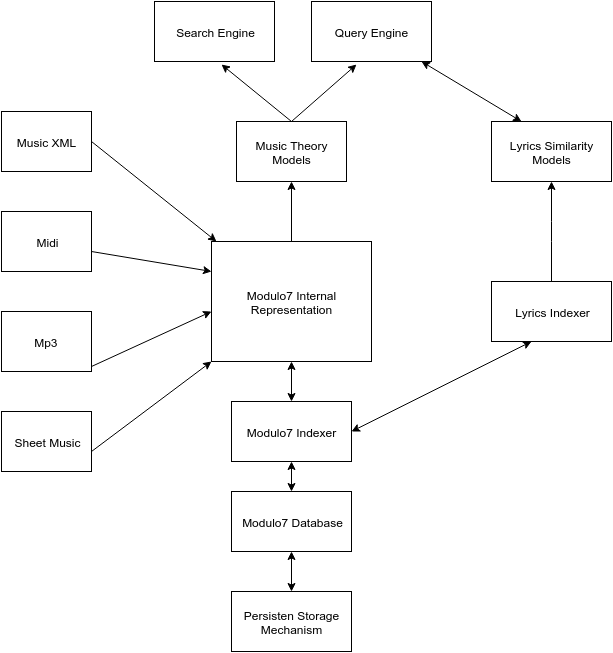
\includegraphics[width=\textwidth]{Modulo7Architecture.png}
\makeatletter
\let\@currsize\normalsize
\caption{Modulo7 architectural design}
\label{fig:Architectural Design}
\end{figure}
\newpage
\section{Client architecture}
\noindent The server exposes a sql like interface as well as a consumable API. Some sample queries would be :-
\begin{enumerate}
\item select midi files from database where $melodic\_complexity > some threshold$
\item select * from database where $artist = led\_zepplin \ and \ harmonic\_movement > harmonic\_movement(stairway\_to\_heaven)$
\item select $ num\_voices \ from \ Database \ where \ songName = someSong.midi$ 
\end{enumerate}

An API will also be exposed to the client along a remote invocation procedure. The API would primarily target single sources for specifics. Some example API would be :-
\begin{enumerate}
\item int getNumVoices(String midiFilePath)
\item double melodicContourMovement(String pngSheetFilePath)
\item double compareAverageAttack(String musicXMLFile)
\end{enumerate}

\noindent This API can be consumed for specific song analysis. As design this API will not work on a bulk of files like its sql counterpart. \\

Moreover the client also exposes a highly customized search engine based on the custom vector space representation of features extracted by Modulo7.

\section{Song sources}
\noindent At the heart of Modulo7's design is its song sources adaptors (or converters) into its own internal binary format. Each music source is a different representation and while certain sources ascribe what how music should be played (e.g musicxml, sheet music), other formats ascribe what is actually being played (e.g midi, mp3). There are many other music sources in existence (e.g guitar tablature, GUIDO format, humdrum format), but for the purposes of breadth and ubiquity, these four sources have been targeted as input for Modulo7. Note that acquiring features from each format is a domain specific challenge and inaccuracies are inherent because of that. The following subsections describe the individual formats in detail and the challenges encountered in parsing them.

\subsection{Midi format}
\noindent MIDI (short for Musical Instrument Digital Interface), is a technical specification for encoding of events on a midi enabled instrument and a protocol for interfacing and communicating between various midi enabled instruments. Typically any midi enabled electronic instrument when played, relays to its internal circuitry a message. Examples of such messages could be a particular note is being hit on a keyboard, a note is being hit off after being hit on, tempo based messages on the number of ticks per second etc. While MIDI is a technical specification for encoding music the score is being played, Modulo7 treats it as a symbolic representation of music. Midi was also a simple and popular encoding format for music and gaming industry in the nineteen ninties. \\\\
A symbolic representation is a codification of music which acts a higher level of abstraction (individual notes or chords being played) as compared to lower level representations like audio files (which codify information like waveforms). Modulo7's internal representation is also a symbolic representation. Symbolic representations are easier to manipulate when applying a music theoretic criteria. \\
Midi is one of the easier formats to parse for musical specifications. Moreover there is a big volunteer community of midi encoders. As such acquiring and parsing non trivial amounts of midi data is not a very challenging task. 

\subsection{Western Sheet Music}
\noindent Sheet music is one of the oldest forms of music in existence. Its a hand written or printed form of music that uses a specific script (a set of musical symbols on a manuscript paper) to ascribe music. Music Composers from Medieval and Modern periods of the western world use western sheet scripting to codify their work while performers play from these sources. A vast body of older work and particularly orchestral work is codified in sheet music. \\

\noindent Like midi, sheet music is also symbolic in nature. However unlike midi, its an expression of how a score should be played, rather than what is being played.  Modulo7 converts digitized versions of these sheet music (e.g sheet music stored .tiff, .png. jpeg etc formats)\\

\begin{figure}
\centering
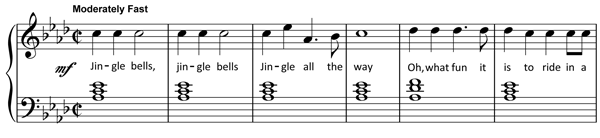
\includegraphics[width=\textwidth]{jingle-bells-sheet-music-piano.png}
\makeatletter
\let\@currsize\normalsize
\caption{Jingle bells melody sheet music representation	}
\label{fig:sheet music example}
\end{figure}

\noindent Parsing digitized sheet music is an extremely challenging task. It requires a solid understanding on Computer Vision and even the state of the art software in existence today cant handle all scores (especially a poorly digitized formats). Given the amount of domain knowledge required, Modulo7 uses a third party library called Audiveris . 

\subsection{Music XML format}
\noindent Music XML format is a standard open format for exchanging digital sheet music. A music XML format is unusual as its a format that is easy to parse for computers and easy for humans to understand it. MusicXML formats are heavily used by music notation applications. Music XML format is a symbolic format and can be considered a modernization of the Sheet music format. Its disadvantage however is unlike sheet music, a performer cant read the piece and play it on the spot directly. \\
Just like Western Sheet music and midi, music XML is a symbolic format as well. Music XML is also a transcription format which specifies how a score should be played. 

\subsection{MP3 format}
\noindent For the sake of completeness, Modulo7 also supports an audio format called mp3. Its an audio encoding format that uses lossy compression to encode audio data. Mp3 gives a reasonably good approximation to other digital audio formats of music storage with a significant savings in space for storage. Its one of the defacto standards of digital music compression and transfer and playback on most digital audio players. 

\section{Modulo7 Internal Representation}

\noindent Modulo7 consists of converters that convert data into Modulo7's internal representation. This representation can be thought of a document representation on which similarity measures described in Chapter 4 can be applied to. Moreover the internal representation can be thought of as an indexed meta data structure for any source of song from which relevant information can be acquired. Hence Modulo7 indexing schematic is a symbolic representation of music much like music xml and sheet music. The converters are responsible for converting different music sources to this representation format. Its important to note that depending on there source one or more of the subcomponents of the internal representation may be missing or wrong. Modulo7 indexes songs based on each of these criteria and on top of these boolean queries can be formulated. The components are broadly categorized as the following:-\\

\noindent \textbf{Song Metadata:} The metadata aspects in a song e.g. The name of the song/ the composer/performer's name, Key Signature of the Song, Meter of the Song etc. These are global properties of the song. \\

\noindent \textbf{Voices in a song:} Similar to the Voices in Music theory, Voices in Modulo7 represent the same symbolic data as is present in the sources from which the information is parsed.\\

\noindent \textbf{Lyrics of a song:} The textual representation (along with delimiters for line breaks) for the lyrics of a song. Lyrics can live independently as separate entities (if the input to Modulo7 is a text file containing the lyrics and no other information). However midi/musicxml and sheet music have optional lyrics elements present in their transcriptions and Modulo7 transcribes from those. \\\\
In most cases though lyrics exists as a separate entity from songs. In such cases, Modulo7 separately indexes lyrics. In certain datasets, the lyrics representation is different (for example the million song dataset has a representation format as a bag of words with counts of the words occuring for each format \cite{msd}). Modulo7 accomodates such formats as well.

\begin{figure}
\centering
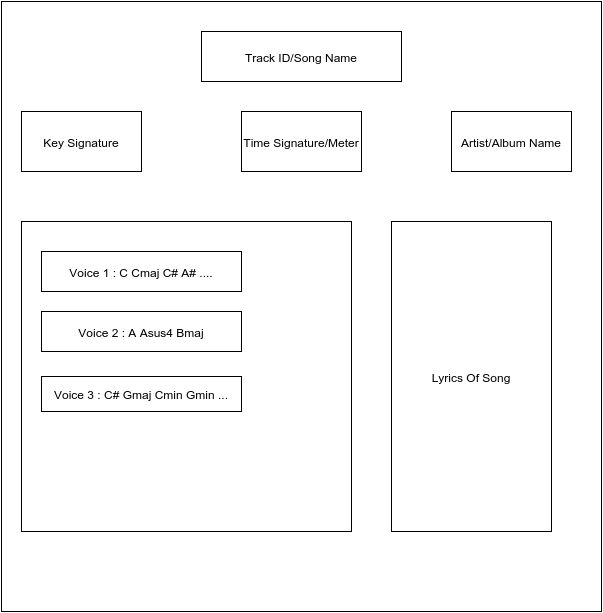
\includegraphics[width=\textwidth]{DocumentStructureOfModulo7.png}
\makeatletter
\let\@currsize\normalsize
\caption{Modulo7 internal representation}
\label{fig:figureDocStruct}
\end{figure}

\section{Methodology}

\noindent This section contains the methodology followed in the information retrieval phase and then the indexing steps taken after the domain specific conversion is completed by Modulo7's adapters

\begin{enumerate}
\item Given a root directory, Modulo7 recursively parses all the sheet music image files, mp3, midi and music xml files. Depending on the file type individual parser modules are invoked and an internal representation is created in memory and serialized to disk (depending on user preference)
\item Modulo7 then indexes all the objects created on specific meta data (such as key signature, time signature and artist of a song). Moreover it also creates a lucene index on lyrics extracted. It stores all these indices in memory. 
\item Modulo7 then exposes a prompt to the consumer which contains a set of standard querying options along with a SQL like querying interface. Consumer can then choose the option they like and query the constructed database.
\end{enumerate}

\subsection{Modulo7 standard query set}

\noindent Modulo7 exposes a standard set of querying features to the consumer. These queries are useful to extract simple information from the parsed dataset from Modulo7. The following are the sample queries that can be relevant for a user :-

\begin{enumerate}
\item Return all songs that are in the key of CMajor
\item Return all songs that are in in the Minor scale
\item Return a ranked order of lyrics given an input string (for example a verse in the song) while treating lyrics like a normal document
\item Return all songs that are performed by Led Zepplin
\item Return all polyphonic songs in the Database
\item Return all music xml files that have been transcribed with a treble clef
\item Return song with a melodic repetition factor above a given thresh hold
\item Return all songs that are of species two counterpoint. 
\end{enumerate}

\noindent The simple query framework has limited expressiveness in querying options but is an example set to the user on what can be queried. Modulo7 also exposes a slightly harder to use SQL like query syntax to concatenate boolean expressions of these example queries and more (boolean combinations of all criteria and statistics defined in criteria \ref{criteria} and statistic \ref{statistic} sections)

\subsection{Modulo7 SQL Language Specifications}

\noindent On top of the standard set of query set defined as an example set, Modulo7 also supports a custom query language for extracting relevant information from a parsed and indexed data set. This language is similar to SQL but its internal processing is radically different. A generic expression can be expressed as follows
\begin{equation}
\textbf{select input\_src\_list  from DATABASENAME where expr\_list}
\end{equation}

\noindent Here input list is a set of music sources to be parsed. An expression list is a boolean conjunctive or distinctive list that outputs a subset of the original set of songs in the database. The definitions for the terms are as follows:-

\begin{enumerate}
\item \textbf{input\_src\_list} : An argument list of all the acceptable formats of is any combination of songs : midi, musicxml, sheet and mp3. This clears out all the formats that are irrelevant to the consumer. 

\item \textbf{DATABASENAME} : The name of the Modulo7 Database. Its an internal consistency check to determine if the consumer is querying against the right Modulo7 database. 

\item \textbf{expr\_list} : A conjunctive and/or disjunctive list of boolean queries on statistics and criteria defined in sections \ref{criteria} and \ref{statistic}. This allows for a greater degree of customization as compared to the other frameworks in literature as well as expose a structured query language for querying (which is sorely lacking in other frameworks). The elements of the expr\_list are defined as follows:-

\begin{enumerate}
\item \textbf{criteria is or is not true} : Returns a subset of songs from a candidate state which either satisfy or dont satisfy a given criteria. The argument criteria is replaced by an implemented criteria in \ref{criteria}
\item \textbf{statistic relational\_op doubleValue} : Returns a subset of a songs from candidate set which satisfy this criteria : When a statistic is applied on a song in a candidate set, the returned value of the statistic satisfies a relational operation to the given value. The arguments to this expression is a statistic implemented in \ref{statistic}, a relational operator and a double value.
\item \textbf{statistic between value1 and value2} : This form is a range query. This query returns the subset of songs from a candidate set which satisfy this criteria : When a statistic is applied on a song in a candidate set, the returned values lies in between value1 and value2. 
\end{enumerate}
\end{enumerate}

\noindent Each of these basic query component returns a subset of songs that satisfy the query component. These query components can be concatenated conjunctively or disjunctively to form a boolean query. So a query is effectively $Q = \cup_i | \cap_i (qc)$, where qc is a query component described above and Q is the resultant query. \\

\subsection{Modulo7 Similarity Engine}

\noindent On top of Modulo 7 supporting custom queries, it also acts in a ranked search engine mode. However the ranking model of the search engine is based on similarity measures based on the structural analysis of the music sources and are described in \ref{similarity}

\subsection{Modulo7 Lyrics Analyzer Architecture} \label{lyricsarch}

\noindent The modulo indexer also indexes lyrics, but treats lyrics objects as text components. So the standard model of text Information Retreival techniques can be used type analyze lyrics. Modulo7 implements lyrics indexing and standard NLP operations on lyrics.

\begin{enumerate}
\item Modulo7 parses lyrics components from some of its sources (for example musicxml and midi have embedded lyrics structures inside it). This is stored along with the song object
\item Modulo7 also parses independent lyrics structures provided to it. This allows for increased flexibility for Modulo7 to just parse lyrics objects
\item Modulo7 creates a lucene index of the lyrics objects once parsed from its sources. This allows for users to make standard text queries via Lucene. 

Modulo7 also provides support for rudimentary Natural Language Processing operations on top of the lyrics obtained. Two supported operations for lyrics are :-
\end{enumerate}

\begin{enumerate}
\item \textbf{Language ID} : Modulo7 can detect what language the song's lyrics is written in. It does this via an language ID call to alchemy \ref{Alchemy}. 
\item \textbf{Sentiment Analysis} : Modulo7 can detect the positivity or negativity sentiment of a song's lyrics and assigns a score to it (with -1 standing for highest degree of negativity and similarly 1 standing for highest degree of positivity). 
\end{enumerate}

\noindent On top of these features, the lyrics analyzer provides support for meta data (also called as tag) prediction. Given a data set with tags annotated to songs along with lyrics, Modulo7 can predict tags for new input lyrics. The following tag estimation schemes are implemented in Modulo7:-

\subsection{Naive Tag Membership}

\noindent Consider $T(S_i)$ be defined as the set of tags for the $S_i$ which is the $i^{th}$ song in the music match dataset. Let $S_{new}$ be a new song for which tags need to be predicted and get L(S) represent the lyrics of a song. Hence $L_{new}$ should be similar to some $L(S_k)$ for their tags to be similar. Let $S_{sim} = {S_i | isSim(S_i, S_new) = true} $ be the set of all the songs similar to $S_new$. We define $T_{new} = \{\cup \ T(S_i) \ | \ S_i \in S_{sim}\}$. In other words the tags of the new song is the union of the tags in the songs similar to the new song. This estimation scheme is called the \textbf{naive tag estimation}. \\\\
This scheme does not capture the strength of similarity a song has to another, or the relative prevalence of tag membership to a song. In order to address this issue, we introduce two non trivial schemes.

\subsection{Weighted Tag Membership}

\noindent In the previous scheme, there are no considerations for the weights associated with the tags. In order to accommodate we assume the existence of tag weights associated for tags in the song meta data. 
set $WT(S_i)$ be defined as set of tag weight pairs (tag with associated weight) for a given song and $w_k$ is the weight of $k^{th}$ tag. Let $WS_{sim} = sort_v({S_i, \alpha_i WT(S_i) | isSim(S_i, S_new) = v})$ be the weighted set of Song and tag pairs where $\alpha_i$ is a scaling factor which is defined $\alpha_i = \frac{sizeof(WT(S_i)) - i}{sizeof(WT(S_i))}$. $\alpha_i$ is a fraction which is multiplied with every weight associated with tags of song $S_i$. \\\\
This scheme takes into account both the rank of the songs in based on a similarity metric and and also the weight associated with each individual tag. The scheme can retain only a subset of the maximal weighted tags in the resulted weighted tag set for the input song.

\subsection{Most frequently occuring tags}

\noindent In the previous scheme, the frequency of tags occurring inside the dataset is ignored. In order to accommodate that let 

\section{Limitations of Modulo7} 

\noindent While Modulo7 attempts to solve a large set of problems (custom query specification based on structuralhe  aspects of music, similarity analysis, logical indexing scheme), there are some fundamental limitations to what Modulo7 can or cannot do. Some of the notable ones are listed as follows:-

\begin{enumerate}
\item Modulo7 does not perform any kind of timbral analysis. This limitation is by design, since all formats of music do not convey timbral information faithfully (for instance sheet music is a specification of music to be played and not an actual recording), hence Modulo7 has not been designed with timbral analysis in mind.
\item Modulo7 does not take into account varying time and/or key signatures. This is due to the fact that in most western music, these two global parameters stay constant for songs.
\item Modulo7 assumes input mp3 files are monophonic. This is due to the fact that the state of the art in audio processing techniques have not solved the problem of polyphonic symbolic transcription faithfully  \cite{melextract}
\item Modulo7 does not mine cultural data or perform any sort of collaborative filtering directly. However it supports meta data estimation based on pre-existing tags in a given lyrics dataset.
\end{enumerate}
